%\documentclass[main]{subfiles}

%\begin{document}

%\appendix

\chapter{GPS - Información adicional}
\label{chap:gps-extra}

\section{Geometría: DOP - \textit{Dilution of precision}}
\label{sec:dop}

\begin{wrapfigure}{r}{0.5\textwidth}
\vspace{-30pt}
  \begin{center}
    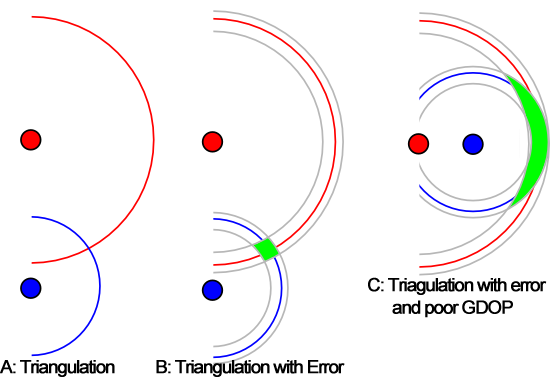
\includegraphics[width=.5\textwidth]{./pics_gps/dop.png}
  \end{center}
\vspace{-20pt}
  \caption{DOP en 2 dimensiones.}
\vspace{-50pt}
\label{fig:dop.png}
\end{wrapfigure}

El método que utiliza el GPS para determinar su ubicación consiste básicamente en:
\begin{enumerate}
\item Determinar la distancia $r_i$ a cada satélite $S_i$, cuya posición es $P_i$.
\item Repetir el paso anterior para cada satélite disponible.
\item Intersectar las ``cáscaras'' de las esferas de centros $P_i$ y radios $r_i$.
\end{enumerate}

Las ``cáscaras'' de las esferas no serán de ancho despreciable, ya que hay un cierta incertidumbre asociado a los datos. Esto implica que la intersección será un volumen, en lugar de un punto. La geometría de la distribución de los satélites determinará el tamaño de este volumen, y por lo tanto la incertidumbre en la determinación de la posición. En la figura \ref{fig:dop.png}\footnote{Imagen obtenida de \href{http://en.wikipedia.org/wiki/Dilution\_of\_precision\_(GPS)}{Wikipedia}} se muestra un ejemplo ilustrativo, en dos dimensiones.

El DOP es el cociente entre la exactitud de la ubicación y exactitud de la medida\cite{bib:sat-pos}:
\begin{equation*}
  \sigma = \sigma_o.DOP
\vspace{-10pt}
\end{equation*}
donde
\begin{itemize}
\item $\sigma$: Exactitud de la medida.
\item $\sigma_o$: Exactitud de la posición. 
\end{itemize}

 Básicamente, el DOP representa la sensibilidad de localización frente a errores en las medidas, o sea, cuanto te vas a perder si te llego una medida equivocada. Cuanto más bajo sea el DOP, mejor. En la tabla \ref{tab:dop} se muestra como interpretar valores típicos\cite{bib:sat-dop-values}.

\begin{table}[H]
\begin{center}
\begin{tabular}{|l|c||p{7cm}|}
\hline
\rowcolor[gray]{0.9}
1 & Ideal & Máxima exactitud posible.\\
\rowcolor[gray]{0.95}
1-2 & Excelente & La exactitud a este nivel se considera suficiente para casi cualquier aplicación.\\
\rowcolor[gray]{0.9}
2-5 & Bueno & Este nivel marca el mínimo apropiado para navegación. \\
\rowcolor[gray]{0.95}
5-10 & Moderado & Las medidas se pueden utilizar, pero es recomendado buscar un lugar con cielo más abierto. \\
\rowcolor[gray]{0.9}
10-20 & Regular & Solo se deben usar los datos para estimaciones de muy poca precisión. \\
\rowcolor[gray]{0.95}
$>$20 & Malo & A este nivel, las exactitud de las medidas puede tener un error de hasta 300m, deben descartarse. \\
\hline
\end{tabular}
\caption{Interpretación de los valores de DOP.}
\label{tab:dop}
\end{center}
\end{table}

El GPS envía información sobre:
\begin{itemize}
\item \textit{HDOP} - DOP horizontal:
  \begin{equation}
    \label{eq:hdop}
    HDOP = \sqrt{\sigma_{easting}^2+\sigma_{northing}^2}    
  \end{equation}
\item \textit{VDOP} - DOP vertical:
  \begin{equation}
    \label{eq:vdop}
    VDOP = \sqrt{\sigma_{altitud}^2}
  \end{equation}
\item \textit{PDOP} - DOP de la posición:
  \begin{equation}
    \label{eq:pdop}
    PDOP = \sqrt{\sigma_{easting}^2+\sigma_{northing}^2 + \sigma_{altitud}^2}
  \end{equation}
\end{itemize}

Esta información se puede utilizar en el algoritmo de control, para ponderar los datos provenientes del GPS.
